%\documentclass[twoside,11pt,openright,a4paper]{report}
\documentclass[a4paper]{article}

\usepackage[utf8]{inputenc}
\usepackage[american]{babel}
\usepackage{svg}
\usepackage{latexsym}
\usepackage{amssymb}
\usepackage{amsmath}
\usepackage{epsfig}
\usepackage[T1]{fontenc}
\usepackage{lmodern}
\usepackage{natbib}
\usepackage[labeled]{multibib}
\usepackage{color}
\usepackage{datetime}
\usepackage{epstopdf}
\usepackage{titling}
\usepackage{listings}
%\usepackage{minted}
\usepackage{graphicx}


\setsvg{svgpath = ../svgs/}

\newenvironment{bottompar}{\par\vspace*{\fill}}{\clearpage}

\makeatletter
\newcommand\csAdvisor[1]{\renewcommand\@csAdvisor{#1}}
\newcommand\@csAdvisor{\@latex@error{No \noexpand\csAdvisor given}\@ehc}

\pretitle{
  \pagestyle{empty}
  \pagenumbering{roman}
  \noindent{\rule{\linewidth}{1mm}\\[1ex]}
  \begin{center}
  \Huge\sf
}
\posttitle{
  \end{center}
}
%\preauthor{}
\postauthor{
  \end{tabular}
  \\[2ex]
  \noindent\rule{\linewidth}{1mm}\\[4ex]
  \noindent{\Large\sf IoT/P2P, Computer Science\\[1ex]}
  \end{center}
}
%\predate{}
\postdate{
  \\[1em]
  {\large Advisor: \@csAdvisor}
  \end{center}
  \begin{bottompar}
  
\epsfig{file=logo.eps}
  \end{bottompar}
}
\makeatother

\newcommand{\todo}[1]{{\color[rgb]{.5,0,0}\textbf{$\blacktriangleright$#1$\blacktriangleleft$}}}

\usepackage{hyperref}

\hypersetup{
    pdfborder = {0 0 0}
}

\begin{document}

%%%%%%%%%%%%%%%%%%%%%%%%%%%%%%%%%%%%%%%%%%%%%%%%%%%%%%%%%%%%%%%%%%%%%%%
\author{Kasper Lynderup - 20105319\\Timothi Hansen - 201303516\\Rohde Fischer - 20052356}
\csAdvisor{Niels Olof Bouvin}
\title{Using solar panels to deduce weather}
\pagestyle{empty}
\maketitle

%%%%%%%%%%%%%%%%%%%%%%%%%%%%%%%%%%%%%%%%%%%%%%%%%%%%%%%%%%%%%%%%%%%%%%%

\pagestyle{plain}
\setcounter{page}{1}

\tableofcontents
\pagenumbering{arabic}
\setcounter{secnumdepth}{2}

%%%%%%%%%%%%%%%%%%%%%%%%%%%%%%%%%%%%%%%%%%%%%%%%%%%%%%%%%%%%%%%%%%%%%%%

\section{Introduction}
Photovoltaic modules (PV), commonly known as solar panels, works by
having two silicon based semiconductors, namely a n-type and a p-type.
The two semiconductors react when exposed to photons which is used to
create electricity \cite{photovoltaic}.

\todo{BAsed on this we want to try to correlate power generated with cloud conditions}


%%% Local Variables:
%%% mode: latex
%%% TeX-master: "thesis"
%%% End:


\section{Related work}
%\subsection{Weather sensing}
There has already been some research in measuring weather data by
utilizing some of the sensor capabilities that arises from the
increasing amount of technology in use.

OpenSignal have created the app WeatherSignal that utilized phone
battery temperatures \citep{temperatures2013} to deduce information
about the air temperature in heavily populated areas.  They proved a
strong relation between the temperature of a the phone batteries and
the outside temperatures.  The authors believe that the data can be
further improved, if the data can be calibrated according to phone
models and if the phone is inside or outside, as heating and air
conditions bias the data.

A correlation between the radio signals used for phones and rain
measurements has also been proved \citep{rainfall2007}.  The radio
signals can be used to measure the amount of rain in between two
points.  The measurements is fairly accurate, and it's assumed that
they can be further improved if improved for the signal loss due to
wet antennas.

It is believe that the combination of various weather sensing
techniques such as \cite{rainfall2007}, \cite{temperatures2013} and
measurement of clouds by PV systems, such as proposed in this article,
is likely to have some useful potential.  For instance the maximum
power point tracking units of PV systems can be improved with weather
data \citep{mppt2004}.

%%% Local Variables:
%%% mode: latex
%%% TeX-command-extra-options: "-shell-escape"
%%% TeX-master: "thesis"
%%% End:


\section{Setup}
Setup which is used in this research paper is very simple. There are actually two setups, because there were a need to record cloud coverage data from somewhere, and at the same time there were a need to record solar panel data.\\ 
First setup which collects solar panel data is placed in a town named Mønsted which can be seen on a picture below. The setup consists of  PV, inverter, and raspberry pi, which collects data into a Sql database. \\
The second setup which records cloud coverage data is placed inside Aarhus university, where a stationary computer is running and gathering data from OpenWeather.com api, and stores the data into separate sql database. Data which is gathered from OpenWeather api are coming from two different towns Stoholm and Karup where both towns are closest to first setups placement, and there are no way to force OpenWeather api to return data from the same town always.\\
At last data from both setups are read into one main DB where data gets treated. 

\begin{figure}[h]
  \centering
 % 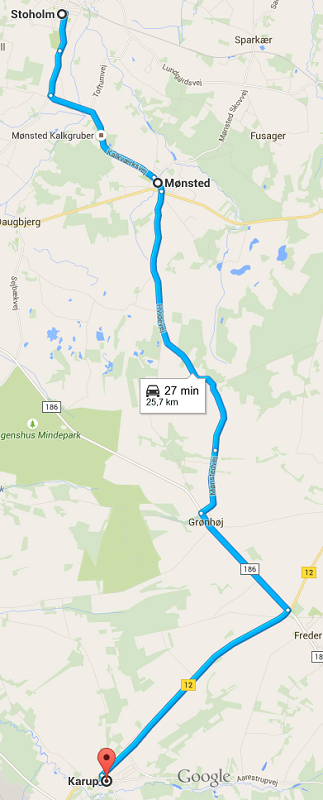
\includegraphics{MapsPicture.png}
 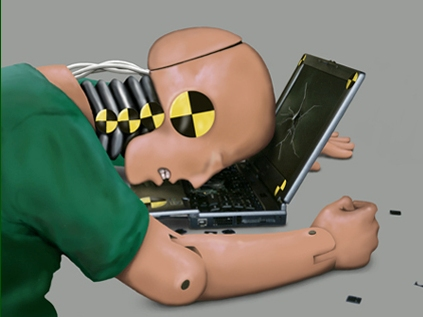
\includegraphics{dummy.jpg}
  \caption{3 towns where data is recorded}
      \label{fig:MapsPicture}
\end{figure}

\section{Data analysis}
From the fact that PV systems is sensitive to the amount of photons
reaching them and that research has shown that larger scale PV systems
and areas can be used to smooth out weather data the expected results
show a clear connection \citep{southafrica, cloudTrack, photovoltaic}.
The approach will be to first off confirm that it's likely to be true
and then refining the data for the purpose to confirm or refute this
hypothesis.

By plotting the raw data
The apparent view of things the data also seem to have a correlation
as can be seen on figure \ref{fig:cloudsAndPower}.  It seems likely
from the graph that there is some correlation, between the clouds and
the PV system, as there's a tendency for the effect to drop when
there's more clouds.

\begin{figure}
  \centering
  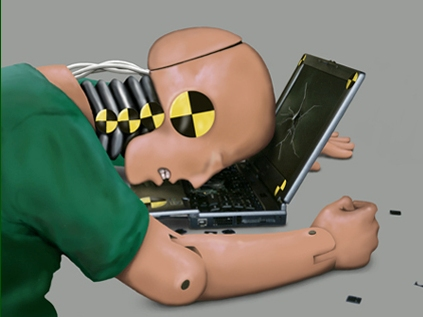
\includegraphics{dummy.jpg}
  \caption{Noisy unfiltered data}
  \label{fig:noise}
\end{figure}

\begin{figure}
  \centering
  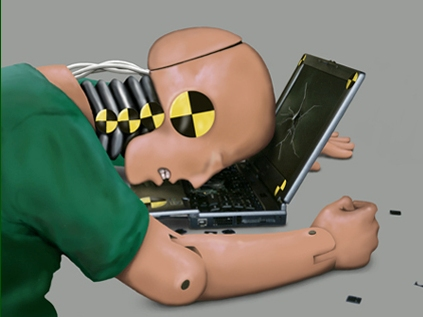
\includegraphics{dummy.jpg}
  \caption{Cloud cover and averages of power generated (10 minute
    intervals)}
  \label{fig:cloudsAndPower}
\end{figure}

However further analysis puts some doubt to that.  The blue line in
figure \ref{fig:cloudsAndPower} shows the optimal effect measured at a
given point of time in the day.  To test that hypothesis a scatter
plot comparing how far from the optimal the power generation is
compared to the cloud coverage.

\begin{figure}[h]
  \centering
  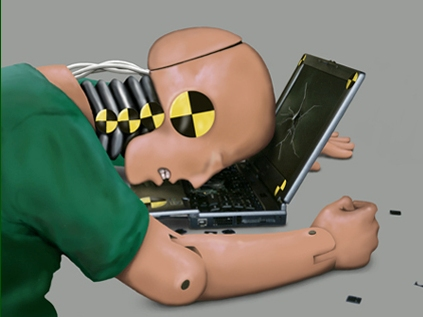
\includegraphics{dummy.jpg}
  \caption{Scatter plot from comparing effect, cloud coverage and
    optimal effect}
  \label{fig:fractiles}
\end{figure}

\todo{Boxplot comments, more analysis}

That a single PV system is very sensitive to even small changes can
easily be seen following the green curve on figure \ref{fig:noise}.
It's apparent from the amount of fluctuations that even small things
can influence the effect.  Both \citep{cloudTrack} and
\citep{southafrica} has data confirming that small scale PV systems
are easily affected by things such as clouds, they still look at large
systems in comparison with a personal system.  Thus it is likely that
even a flock of birds can influence it.

A larger area of PV systems and bigger PV systems can smooth out noise
in the data \citep{southafrica,cloudTrack}.  The effect of larger
systems could be interesting if they can be accessed, for the approach
of this project it would be an interesting addition to get access to
more systems.  The approach to have a larger area of PV systems is
used is used to try and even out all noise caused from clouds
\citep{southafrica}, where the intend here would be to even out some,
such that conclusions about correlation about the weather and effect
can be made.  The fact that the weather impact can be smoothed a lot,
when it's done over areas of 250x250 and 500x500 km squares, but
weather data is still quite apparent on 50x50 km squares
\citep{southafrica}, indicates both that a larger area than a single
PV system will smooth the data, but without loosing the stronger
connection with weather data as long as the area is relatively small.

%%% Local Variables:
%%% mode: latex
%%% TeX-command-extra-options: "-shell-escape"
%%% TeX-master: "thesis"
%%% End:


\section{Improvements}
PV systems react to photons and thus are affected by clouds
and atmospheric disturbances.  This gives an indication that we should be able to make
a connection between clouds and the effect of the panels
\citep{photovoltaic}.  This claim is further backed by research being
done to even out the noise from weather conditions, most notably
clouds \citep{southafrica, cloudTrack}.  However the fact that the
data analysis contrasts this leaves out three possible conclusions: 1)
there actually is no such connection, 2) clouds do impact but too many
other factors impact it to make any reliable information from clouds
alone, and 3) there are errors in the way the data is collected.  As
option 1 seems very unlikely, both from the science behind PV systems
and that research groups seem to be able to prove this
\citep{southafrica, cloudTrack, photovoltaic}, it seems appropriate to
take a look at option 2 and 3.

Considering that there may be too many data influencing the
measurements, as to cloud coverage by itself being a too small factor
to actually show the intended connection between cloud coverage and
the effect of the system, there is a few options to remedy this.  From
the fact that temperature impacts the amount of power a PV system
produces \citep{mppt2004} taking further account of these data may
show an improvement.  This suspicion however is weakened from the mean
and deviation plots in figure \ref{fig:stat0610}, \ref{fig:stat1014}
and \ref{fig:stat1418}, as the temperature should even out when using
measurements at the same times of the day.  The data on that account
though is in no way conclusive, and a further investigation into it
would require a lot more data than available in this study.

That a single PV system is very sensitive to even small changes can
easily be seen following the green curve on figure \ref{fig:noise}.
It's apparent from the amount of fluctuations that even small things
can influence the effect.  Attempts to even out the effect from
weather conditions, has successfully shown that both larger PV systems
and larger area coverage can be used to smoothe the data from weather
conditions \citep{cloudTrack,southafrica}.  This indicates that using
more PV systems could be useful.  Since the target here isn't to
completely even the data out, the balance between still having data
and reducing the noise from the data gathered should be takin into
consideration.

The approach of having a larger area of PV systems is used to try and
even out all noise caused from clouds.  Using large areas with
multiple PV systems shows that areas of 250x250 and 500x500 km squares
even out very large amounts of the data, but weather data is still
quite apparent on 50x50 km squares \citep{southafrica}.  This
indicates that using a larger area with more PV systems is a viable
approach.  Doing this in a small city such as the one where the
experiment is done would be fairly easy provided that people would
allow collection of their data.

Considering the claim that 1 MW solar panels respond rapidly to
changes in available sunlight \citep{cloudTrack} it is quite likely
that the data in the experiment is simply too sensitive.
The usage of larger PV systems isn't a likely approach if using
peoples personal systems on their roofs, since a personal system in
Denmark is allowed to be max 3 kW, which is a fair deal lower than the
1 MW system.  This however indicates that even very small disturbances
will have an effect on the solar panels and thus simply renders faulty
data.

Another possible cause for faulty data is the lack of precision of the
weather data.  The data given for free from OpenWeatherMap.org is
guaranteed to be updated approximately every 2 hours (they may do it
more often).  Also the weather station doing the measurement isn't
located exactly where the PV system is.  So it is quite possible that
the ground truth data simply isn't reliable enough.

On a final note it would also be an improvement to have data over a
longer period of time, as this would assist in either making it
certain that the noise is either consistent or that it would over time
start to show stronger tendencies towards a connection.

There is plenty of room for improving the data gathered, both by
trying to reduce the chance for potential direct errors but also to
make other effects more apparent.  From the data gathered here, it is too
early to conclude the lack of a connection between clouds and the
effect from solar panels.

Another point of improvements is to actually find out the role of the sun in energy production of PV, because every PV have an optimal sun angle where they receive optimal amount of sun light.  Since the optimal angle of the sun is known, the placement of the sun on the sky at gathered data points can be found, to calculate if there is actually a link between the angle of the sun and PV power generation.

%%% Local Variables:
%%% mode: latex
%%% TeX-command-extra-options: "-shell-escape"
%%% TeX-master: "thesis"
%%% End:


\section{Conclusion}
The effect data from the solar panels turned out to contain too much
noise to draw any useful conclusions.  Despite the fact that no clear
connection has been found there are a lot of ways that conditions for
data analysis can be improved.  Thus it is likely that refinement of
the conditions given will provide a better basis for analysis.
Especially considering the fact that other research projects has seen
a clear connection between clouds and PVs, improving the system with
more PVs for data aggregation and smoothing out noise would be a
logical next step to improve this research.

%%% Local Variables:
%%% mode: latex
%%% TeX-command-extra-options: "-shell-escape"
%%% TeX-master: "thesis"
%%% End:


%%%%%%%%%%%%%%%%%%%%%%%%%%%%%%%%%%%%%%%%%%%%%%%%%%%%%%%%%%%%%%%%%%%%%%%

\section{Acknowledgments}

\begin{itemize}
\item Niels Olof Bouvin and Matthias Nielsen - Guidance and help
  during the project
\item Karl Fischer - Guidance on the physics and chemistry behind
  photovoltaic systems
\item Jan Jensen - Provided access to solar panels
\item Peter Laursen, Mathias Mikkelsen, Karl Fischer - Correction and feedback on the report
\end{itemize}

%%%%%%%%%%%%%%%%%%%%%%%%%%%%%%%%%%%%%%%%%%%%%%%%%%%%%%%%%%%%%%%%%%%%%%%

%\addcontentsline{toc}{chapter}{Primary Bibliography}
\bibliographystyle{alpha}
\bibliography{refs}

\end{document}

%%% Local Variables:
%%% mode: latex
%%% TeX-command-extra-options: "-shell-escape"
%%% TeX-master: t
%%% End: